% Provenance (never printed): cycle 4 (geographie and SVT, "La planete Terre"):
% why a flat map distorts, projections, scale, topographic maps and
% profiles, satellite images and satellite positioning; see
% sources/book1/PROVENANCE.md. Book 1, grade 9, chapter 5.
% Vocabulary guard: owns map projection (Mercator, equal-area), numerical
% scale and scale bar, topographic map, contour line and contour interval,
% remote sensing and satellite image, satellite positioning. "Scale" itself
% is g2's (drawing-to-map, Sync 1 ruling); globe and world map are g3's;
% parallels, meridians, latitude and longitude are g6's; altitude, relief
% and physical map are g4's; slope as a percentage was used in g9.2. The
% speed of light is the physics books' (recalled in prose). The V-rule of
% geological maps belongs to Book 3.
\chapter{خرائط الأرض كلها}\label{ch:g9:maps-of-the-earth}

في كثير من خرائط الجدران المدرسية، تبدو غرينلاند بحجم إفريقيا تقريبًا.
أما على \omterm{def:g3:continents-and-oceans:globe}{مجسم الكرة الأرضية}، فإفريقيا أكبر بنحو أربع عشرة مرة: نحو
29~مليون كيلومتر مربع للبر الإفريقي الرئيسي، مقابل نحو 2.1~مليون
لغرينلاند. وكلتا الصورتين صورة صادقة للأرض، صُنعت بعناية. فأيهما تكذب،
ولماذا؟
% ledger: data:ne-land (areas computed in figdata/grade-9/projections.py)

\begin{recall}
\omterm{def:g2:drawing-to-map:map}{الخريطة} رسم لمكان كما يُرى من أعلى، أصغر من المكان، لها \omterm{def:g2:drawing-to-map:legend}{مفتاح} \omterm{def:g2:drawing-to-map:scale}{ومقياس
رسم} (\cref{ch:g2:drawing-to-map}). \omterm{def:g3:continents-and-oceans:globe}{ومجسم الكرة الأرضية} نموذج صغير للأرض
المستديرة؛ \omterm{def:g3:continents-and-oceans:world-map}{وخريطة العالم} تُظهر الأرض كلها مسطحة، في صورة واحدة
(\cref{ch:g3:continents-and-oceans}). \omterm{def:g6:latitude-longitude:latitude}{ودوائر العرض} \omterm{def:g6:latitude-longitude:longitude}{وخطوط الزوال} تعطي كل
مكان عرضه الجغرافي وطوله الجغرافي (\cref{ch:g6:latitude-longitude}).
\omterm{def:g4:world-physical-map:altitude}{والارتفاع} هو العلو فوق \omterm{def:g4:world-physical-map:altitude}{مستوى سطح البحر}، \omterm{def:g4:world-physical-map:physical-map}{والخريطة الطبيعية} تُظهر \omterm{def:g4:world-physical-map:relief}{التضاريس}
بالألوان (\cref{ch:g4:world-physical-map}). وفي الفيزياء، تتعلم أن الضوء
ينتقل بسرعة نحو \qty{300000}{km} في الثانية.
\end{recall}
% ledger: const:c

\section{لماذا يجب أن تشوّه الخريطة المسطحة}

حاول أن تبسط قشر برتقالة على طاولة: فإما أن يتمزق وإما أن يتمدد. فسطح
الكرة لا يمكن بسطه دون تغيير بعض الأطوال. ولرسم الأرض كلها على ورقة،
يختار راسم الخرائط قاعدة ترسل كل نقطة من الكرة الأرضية إلى نقطة من
الورقة، ويختار ما ستحفظه \omterm{def:g2:drawing-to-map:map}{الخريطة} صحيحًا، وما ستتخلى
عنه.

\begin{definition}[الإسقاط الخرائطي]\label{def:g9:maps-of-the-earth:projection}
\emph{الإسقاط الخرائطي}\index{إسقاط خرائطي} قاعدة ترسل كل نقطة من الكرة
الأرضية، معطاة بعرضها وطولها الجغرافيين، إلى نقطة من \omterm{def:g2:drawing-to-map:map}{خريطة} مسطحة. ففي
\emph{إسقاط مركاتور}\index{إسقاط مركاتور}، تكون \omterm{def:g6:latitude-longitude:latitude}{دوائر العرض} \omterm{def:g6:latitude-longitude:longitude}{وخطوط الزوال}
خطوطًا مستقيمة تتقاطع بزوايا قائمة، ويُحفظ شكل كل منطقة صغيرة، لكن
المساحات تُكبَّر أكثر فأكثر كلما اقتربنا من \omterm{def:g3:continents-and-oceans:poles}{القطبين}. وفي
\emph{الإسقاط المتساوي المساحة}\index{إسقاط متساوي المساحة}، تحفظ كل
منطقة مساحتها الحقيقية مقارنةً بالمناطق الأخرى، لكن الأشكال تنثني، أكثر
فأكثر كلما اقتربنا من أطراف
\omterm{def:g2:drawing-to-map:map}{الخريطة}.
\end{definition}

يرسم الشكل أدناه الدوائر المتساوية نفسها على الكرة الأرضية، وكلها بالحجم
نفسه، على الخريطتين. ففي \omterm{def:g2:drawing-to-map:map}{خريطة} مركاتور، تبقى الدوائر مستديرة لكنها تكبر
نحو \omterm{def:g3:continents-and-oceans:poles}{القطبين}: فعند \omterm{def:g6:latitude-longitude:latitude}{خط العرض} \ang{60}، تبلغ مساحتها أربعة أضعاف ما هي عليه
عند \omterm{def:g3:continents-and-oceans:equator}{خط الاستواء}، وقرب وسط غرينلاند، عند نحو \ang{72}، نحو عشرة أضعاف.
وفي \omterm{def:g2:drawing-to-map:map}{الخريطة} المتساوية المساحة، تحفظ الدوائر كلها المساحة نفسها، لكن
البعيدة منها عن المركز تنضغط فتصير أشكالًا بيضوية.
% ledger: data:ne-land (circles and factors computed in figdata/grade-9/projections.py, mercator_area_factor)

ليس هناك إسقاط هو الأفضل لكل شيء. فقد صُنع \omterm{def:g9:maps-of-the-earth:projection}{إسقاط مركاتور} للبحارة:
فالمسار الذي يحافظ على اتجاه البوصلة نفسه خط مستقيم عليه. ولمقارنة
مساحات البلدان أو الغابات أو \omterm{def:g5:weather-and-climate:desert}{الصحارى}، تقول \omterm{def:g2:drawing-to-map:map}{الخريطة} المتساوية المساحة
الحقيقة. وقبل الوثوق \omterm{def:g3:continents-and-oceans:world-map}{بخريطة للعالم}، يجدر السؤال عن الإسقاط الذي
تستعمله.

\begin{omfigure}
\begin{tikzpicture}
\begin{axis}[name=merc, x=0.0215cm, y=0.0215cm, xmin=-180, xmax=180,
  ymin=-140, ymax=169, axis line style={black!50}, ticks=none,
  title={\footnotesize إسقاط مركاتور}, title style={yshift=-1ex}]
  \addplot[black!15, line width=0.3pt] table {figdata/out/grade-9-projections-merc-grid.dat};
  \addplot[fill=black!25, draw=black!45, line width=0.15pt] table {figdata/out/grade-9-projections-merc-land.dat};
  \addplot[fill=orange!55, draw=orange!70!black, line width=0.3pt] table {figdata/out/grade-9-projections-merc-greenland.dat};
  \addplot[fill=blue!30, draw=blue!60!black, line width=0.3pt] table {figdata/out/grade-9-projections-merc-africa.dat};
  \addplot[red!80!black, line width=0.6pt] table {figdata/out/grade-9-projections-merc-circles.dat};
\end{axis}
\begin{axis}[at={(merc.east)}, anchor=west, xshift=0.3cm, x=0.025cm, y=0.025cm,
  xmin=-165, xmax=165, ymin=-83, ymax=83, hide axis,
  title={\footnotesize إسقاط متساوي المساحة}, title style={yshift=-1ex}]
  \addplot[black!15, line width=0.3pt] table {figdata/out/grade-9-projections-moll-grid.dat};
  \addplot[fill=black!25, draw=black!45, line width=0.15pt] table {figdata/out/grade-9-projections-moll-land.dat};
  \addplot[fill=orange!55, draw=orange!70!black, line width=0.3pt] table {figdata/out/grade-9-projections-moll-greenland.dat};
  \addplot[fill=blue!30, draw=blue!60!black, line width=0.3pt] table {figdata/out/grade-9-projections-moll-africa.dat};
  \addplot[red!80!black, line width=0.6pt] table {figdata/out/grade-9-projections-moll-circles.dat};
\end{axis}
\end{tikzpicture}

{\small العالم نفسه في إسقاطين. بالأحمر: دوائر بالحجم نفسه على الكرة
الأرضية، مراكزها كل \ang{30} من \omterm{def:g6:latitude-longitude:latitude}{العرض} و\ang{60} من \omterm{def:g6:latitude-longitude:longitude}{الطول}. بالبرتقالي:
غرينلاند؛ وبالأزرق: البر الإفريقي الرئيسي. في \omterm{def:g2:drawing-to-map:map}{خريطة} مركاتور (يسارًا،
مقطوعة عند \ang{80} جنوبًا و\ang{84} شمالًا، إذ سيكون القطبان على بعد لا
نهائي)، تبدوان بالحجم نفسه تقريبًا؛ وفي \omterm{def:g2:drawing-to-map:map}{الخريطة} المتساوية المساحة
(يمينًا)، إفريقيا أكبر بنحو 14 مرة، كما على الكرة الأرضية. خطوط السواحل من بيانات ناتشورال إيرث.}
% ledger: data:ne-land
\label{fig:g9:maps-of-the-earth:projections}
\end{omfigure}

\begin{example}[غرينلاند وإفريقيا]
يغطي البر الإفريقي الرئيسي نحو 29~مليون~\unit{km^2}، وغرينلاند نحو
2.1~مليون~\unit{km^2}: $29 \div 2.1 \approx 14$. وإفريقيا تمتد على جانبي
\omterm{def:g3:continents-and-oceans:equator}{خط الاستواء}، حيث لا يكاد \omterm{def:g9:maps-of-the-earth:projection}{إسقاط مركاتور} يكبّر شيئًا، بينما يقع معظم
غرينلاند بين نحو \ang{60} و\ang{84} شمالًا، حيث تُكبَّر المساحات من 4 إلى
أكثر من 10 أضعاف. وفي \omterm{def:g2:drawing-to-map:map}{خريطة} مركاتور، تظهر الاثنتان بالحجم نفسه
تقريبًا.
\end{example}
% ledger: data:ne-land (areas and ratios computed in figdata/grade-9/projections.py, areas)

\section{مقياس الرسم}

\omterm{def:g2:drawing-to-map:map}{خريطة} \omterm{def:g1:landscapes-around-us:landform}{وادٍ} أو بلدة قطعة صغيرة جدًا من الأرض حتى إن الإسقاط لا يكاد يهم.
وما يهم هو كم تصغر \omterm{def:g2:drawing-to-map:map}{الخريطة} عن
الأرض.

\begin{definition}[المقياس العددي والمقياس الخطي]\label{def:g9:maps-of-the-earth:numerical-scale}
\emph{المقياس العددي}\index{مقياس عددي} \omterm{def:g2:drawing-to-map:map}{لخريطة} نسبة مثل
$1 : 25\,000$: فالسنتيمتر الواحد على \omterm{def:g2:drawing-to-map:map}{الخريطة} يمثل \num{25000}
سنتيمتر على الأرض، وكذلك لأي وحدة. و\emph{المقياس الخطي}\index{مقياس خطي}
مسطرة مرسومة على \omterm{def:g2:drawing-to-map:map}{الخريطة}، معلَّمة بالمسافات على
الأرض.
\end{definition}

\begin{method}[استعمال المقياس العددي]
\begin{enumerate}
  \item قس المسافة على \omterm{def:g2:drawing-to-map:map}{الخريطة}، بالسنتيمترات.
  \item اضربها في العدد الذي بعد النقطتين: فالنتيجة هي المسافة على
        الأرض، بالسنتيمترات.
  \item حوّل: اقسم على 100 للحصول على الأمتار، وعلى \num{100000} للحصول على الكيلومترات.
\end{enumerate}
\end{method}

\begin{example}[نزهة على خريطة بمقياس $1 : 25\,000$]
على \omterm{def:g2:drawing-to-map:map}{خريطة} بمقياس $1 : 25\,000$، يبلغ طول درب \qty{6}{cm}. وعلى الأرض،
يبلغ $6 \times 25\,000 = \num{150000}$~cm، أي \qty{1500}{m} أو
\qty{1.5}{km}. وكل سنتيمتر من \omterm{def:g2:drawing-to-map:map}{الخريطة} يمثل \qty{250}{m}.
\end{example}

\omterm{def:g9:maps-of-the-earth:numerical-scale}{للمقياس الخطي} ميزة على \omterm{def:g9:maps-of-the-earth:numerical-scale}{المقياس العددي}: فحين تُكبَّر \omterm{def:g2:drawing-to-map:map}{الخريطة} أو تُصغَّر
على شاشة أو آلة نسخ، تُكبَّر المسطرة أو تُصغَّر معها فتبقى صحيحة، بينما
تصير النسبة المطبوعة في الزاوية
خاطئة.

\section{الخريطة الطبوغرافية}

تُظهر \omterm{def:g4:world-physical-map:physical-map}{الخريطة الطبيعية} \omterm{def:g4:world-physical-map:relief}{التضاريس} بالألوان. أما \omterm{def:g2:drawing-to-map:map}{خريطة} منطقة صغيرة فتُظهرها
بدقة أكبر بكثير، بالخطوط.

\begin{definition}[الخريطة الطبوغرافية]\label{def:g9:maps-of-the-earth:topographic-map}
\emph{الخريطة الطبوغرافية}\index{خريطة طبوغرافية} \omterm{def:g2:drawing-to-map:map}{خريطة} مفصلة لمنطقة
صغيرة، بمقياس مثل $1 : 25\,000$ أو $1 : 50\,000$، تُظهر شكل الأرض
وارتفاعها، مع \omterm{def:g1:landscapes-around-us:water}{الأنهار} والطرق والدروب والمباني
والغابات.
\end{definition}

\begin{definition}[خط الكنتور والفاصل الكنتوري]\label{def:g9:maps-of-the-earth:contour}
\emph{خط الكنتور}\index{خط كنتور} خط على \omterm{def:g2:drawing-to-map:map}{الخريطة} يصل بين نقاط من الأرض
لها \omterm{def:g4:world-physical-map:altitude}{الارتفاع} نفسه. و\emph{الفاصل الكنتوري}\index{فاصل كنتوري} هو الفرق في
\omterm{def:g4:world-physical-map:altitude}{الارتفاع} بين خطي كنتور متجاورين؛ وهو نفسه في \omterm{def:g2:drawing-to-map:map}{الخريطة}
كلها.
\end{definition}

تخيّل \omterm{def:g1:landscapes-around-us:landform}{تلة} تقطعها مستويات أفقية، واحد كل \qty{100}{m}. فكل مقطع يقطع
\omterm{def:g1:landscapes-around-us:landform}{التلة} على طول خط مغلق؛ ومن أعلى، تكون هذه الخطوط خطوط
الكنتور.

\begin{omfigure}
\begin{tikzpicture}[font=\footnotesize]
  % side view
  \fill[black!13] (0,0) .. controls (1.2,0.3) and (2.0,1.3) .. (2.8,2.2)
     .. controls (3.2,2.6) and (3.5,2.6) .. (3.7,2.2) .. controls (3.9,1.6) and (4.1,0.4) .. (4.5,0) -- cycle;
  \draw[black!70] (0,0) .. controls (1.2,0.3) and (2.0,1.3) .. (2.8,2.2)
     .. controls (3.2,2.6) and (3.5,2.6) .. (3.7,2.2) .. controls (3.9,1.6) and (4.1,0.4) .. (4.5,0);
  \draw[black!70] (-0.3,0) -- (4.9,0);
  \foreach \y/\h in {0.6/100, 1.2/200, 1.8/300} {
    \draw[omContour, dashed] (-0.3,\y) -- (4.9,\y);
    \node[anchor=east, omContour] at (-0.3,\y) {\h~m};
  }
  \node[anchor=south] at (3.3,2.5) {منظر جانبي};
  \node[anchor=north] at (1.4,-0.05) {منحدر غربي لطيف};
  \node[anchor=north] at (4.1,-0.05) {منحدر شرقي شديد};
  % map view
  \begin{scope}[xshift=8.4cm, yshift=1.3cm]
    \draw[omContour, line width=0.5pt] (0.25,0) ellipse (2.1 and 1.25);
    \draw[omContour, line width=0.5pt] (0.75,0.02) ellipse (1.3 and 0.9);
    \draw[omContour, line width=0.5pt] (1.05,0.04) ellipse (0.62 and 0.5);
    \fill (1.25,0.05) circle (0.04);
    \draw[black!60] (1.25,0.05) -- (2.9,-0.6) node[anchor=west, inner sep=1.5pt] {القمة};
    \node[omContour, fill=white, inner sep=0.5pt] at (-1.85,0) {100};
    \node[omContour, fill=white, inner sep=0.5pt] at (-0.55,0) {200};
    \node[omContour, fill=white, inner sep=0.5pt] at (0.43,0) {300};
    \node[anchor=north] at (0.25,-1.35) {منظر من أعلى: خطوط الكنتور};
    \draw[->] (2.7,0.9) -- (2.7,1.4) node[above] {ش};
  \end{scope}
\end{tikzpicture}

{\small \omterm{def:g1:landscapes-around-us:landform}{تلة} مقطوعة كل \qty{100}{m} (رسم تخطيطي). من أعلى، يعطي كل مقطع
\omterm{def:g9:maps-of-the-earth:contour}{خط كنتور} مغلقًا حول القمة. وحيث يكون الانحدار شديدًا (في الشرق)،
تتقارب الخطوط؛ وحيث يكون لطيفًا (في الغرب)،
تتباعد.}
\label{fig:g9:maps-of-the-earth:slices}
\end{omfigure}

تُقرأ \omterm{def:g9:maps-of-the-earth:topographic-map}{الخريطة الطبوغرافية} ببضع قواعد.
\begin{itemize}
  \item خطوط الكنتور لا تتقاطع أبدًا: فللنقطة \omterm{def:g4:world-physical-map:altitude}{ارتفاع} واحد فقط.
  \item كلما تقاربت خطوط الكنتور، اشتد الانحدار؛ وإذا تباعدت، كانت الأرض
        لطيفة الانحدار؛ وإذا غابت الخطوط، كانت شبه مستوية.
  \item الخطوط المغلقة المتداخلة بعضها في بعض، التي يزداد ارتفاعها نحو
        الداخل، تدل على \omterm{def:g1:landscapes-around-us:landform}{تلة}؛ وكثيرًا ما تُعلَّم قمتها بنقطة مع ارتفاعها،
        وهي \emph{نقطة الارتفاع}.
  \item حيث يعبر \omterm{def:g9:maps-of-the-earth:contour}{خط كنتور} \omterm{def:g1:landscapes-around-us:landform}{واديًا}، ينثني نحو المنبع، على شكل حرف V
        يشير نحو رأس \omterm{def:g1:landscapes-around-us:landform}{الوادي}.
  \item كل خامس خط، وهو \emph{\omterm{def:g9:maps-of-the-earth:contour}{خط الكنتور} الرئيسي}، يُرسم أغلظ ويُكتب
        عليه ارتفاعه.
\end{itemize}

انحدار الأرض بين نقطتين هو الارتفاع مقسومًا على المسافة الأفقية، ويُكتب
كثيرًا نسبةً مئوية. وفي \omterm{def:g2:drawing-to-map:map}{الخريطة} أدناه، بالاتجاه شمالًا من \omterm{def:g1:landscapes-around-us:water}{النهر}، يبعد
خطا الكنتور \qty{200}{m} و\qty{400}{m} على الخط C--D أحدهما عن الآخر
نحو \qty{0.75}{km}: فالانحدار نحو $200 \div 750
\approx 0.27$، أي \qty{27}{\%}.
% ledger: (invented region: crossings 2.09 and 2.83 km from C, figdata/grade-9/varden_topo.py)

\begin{method}[رسم مقطع طبوغرافي]
\begin{enumerate}
  \item ارسم خط المقطع على \omterm{def:g2:drawing-to-map:map}{الخريطة}، من طرف (C) إلى الطرف
        الآخر (D).
  \item ضع الحافة المستقيمة لشريط من الورق على طول الخط؛ وعلّم C وD،
        وكل نقطة يعبر فيها الخط \omterm{def:g9:maps-of-the-earth:contour}{خط كنتور}، مع
        ارتفاعها.
  \item ارسم محورًا أفقيًا بطول C--D (المسافات) ومحورًا رأسيًا
        للارتفاعات.
  \item انقل كل علامة إلى الرسم البياني، عند مسافتها من C وعند
        ارتفاعها، وصِل النقاط بمنحنى أملس: مستديرًا عند قمم \omterm{def:g1:landscapes-around-us:landform}{التلال}،
        ومستويًا على طول قاع \omterm{def:g1:landscapes-around-us:landform}{الوادي}.
\end{enumerate}
\end{method}

\begin{omfigure}
\begin{tikzpicture}
\begin{axis}[name=map, x=2cm, y=2cm, xmin=2, xmax=8, ymin=1.8, ymax=6.2, ticks=none,
  axis line style={black!60}, clip mode=individual]
  \addplot[contour] table {figdata/out/shared-region-contours.dat};
  \addplot[index contour] table {figdata/out/shared-region-index-contours.dat};
  \addplot[river] table {figdata/out/shared-region-river.dat};
  \addplot[only marks, mark=none, point meta=explicit symbolic, nodes near coords,
    nodes near coords align={center}, nodes near coords style={font=\tiny, fill=white, inner sep=0.6pt, text=omContour}]
    table[meta=label] {figdata/out/grade-9-varden_topo-labels.dat};
  \addplot[only marks, mark=*, mark size=1.2pt, point meta=explicit symbolic, nodes near coords,
    nodes near coords align={right}, nodes near coords style={font=\scriptsize, inner sep=1.5pt}]
    table[meta=label] {figdata/out/grade-9-varden_topo-spots.dat};
  \addplot[black, line width=0.8pt] table[x=x_km, y=y_km] {figdata/out/grade-9-varden_topo-cd.dat};
  \addplot[only marks, mark=none, point meta=explicit symbolic, nodes near coords,
    nodes near coords align={left}, nodes near coords style={font=\small\bfseries, inner sep=2pt}]
    table[meta=label] {figdata/out/grade-9-varden_topo-cd.dat};
  \coordinate (na) at (axis cs:8.3,5.3);
  \coordinate (sb) at (axis cs:2.2,1.95);
\end{axis}
\pic at (na) {northarrow};
\fill[white] ($(sb)+(-0.1,-0.42)$) rectangle ($(sb)+(2.3,0.25)$);
\pic at (sb) {scalebar={2}{1 km}};
\node[anchor=west, font=\footnotesize, fill=white, inner sep=1pt] at ($(sb)+(2.35,0.06)$) {$1 : 50\,000$};
\begin{axis}[at={(map.south)}, anchor=north, yshift=-0.9cm, x=2cm, y=0.006cm, clip=false,
  xmin=0, xmax=4, ymin=100, ymax=600, axis x line=bottom, axis y line=left,
  axis line style={-}, grid=major, grid style={black!12},
  xtick={0,1,2,3,4}, ytick={100,200,...,600}, tick label style={font=\scriptsize},
  xlabel={\foreignlanguage{arabic}{المسافة من C \babelsublr{(km)}}}, ylabel={\foreignlanguage{arabic}{الارتفاع \babelsublr{(m)}}}, label style={font=\footnotesize}]
  \addplot[black!70, line width=0.8pt] table[x=s_km, y=z_m] {figdata/out/grade-9-varden_topo-profile.dat};
  \addplot[only marks, mark=*, mark size=1.1pt, omContour] table[x=s_km, y=z_m] {figdata/out/grade-9-varden_topo-cross.dat};
  \node[font=\small\bfseries, anchor=south] at (axis cs:0,600) {C};
  \node[font=\small\bfseries, anchor=south] at (axis cs:4,600) {D};
\end{axis}
\end{tikzpicture}

{\small في الأعلى: \omterm{def:g9:maps-of-the-earth:topographic-map}{خريطة طبوغرافية} لجزء من تلال فاردن بمقياس $1 : 50\,000$
(\qty{1}{cm} على \omterm{def:g2:drawing-to-map:map}{الخريطة} لكل \qty{500}{m} على الأرض). \omterm{def:g9:maps-of-the-earth:contour}{الفاصل الكنتوري}
\qty{50}{m}؛ وخطوط الكنتور الرئيسية، وهي أغلظ، عند 250 و\qty{500}{m}.
ويجري \omterm{def:g1:landscapes-around-us:water}{النهر} شرقًا على طول قاع \omterm{def:g1:landscapes-around-us:landform}{وادٍ} مستوٍ. في الأسفل: المقطع الطبوغرافي
على طول C--D، من الجنوب إلى الشمال؛ والنقاط هي حيث يعبر C--D \omterm{def:g9:maps-of-the-earth:contour}{خط كنتور}
(المقياس الرأسي ممطوط ثلاث مرات).}
% ledger: (invented region: the Varden Hills, figdata/shared/region.py; labels, spot height and profile from figdata/grade-9/varden_topo.py)
\label{fig:g9:maps-of-the-earth:topo}
\end{omfigure}

\section{صور الأقمار الصناعية للأرض}

في 23~يوليو 1972، أطلق صاروخ أول قمر صناعي بُني لدراسة سطح الأرض، وسُمّي
لاحقًا لاندسات~1. وكان يدور حول الأرض 14 مرة في اليوم على \omterm{def:g4:world-physical-map:altitude}{ارتفاع}
\qty{917}{km}، من \omterm{def:g3:continents-and-oceans:poles}{قطب} إلى \omterm{def:g3:continents-and-oceans:poles}{قطب}، فيمر فوق المكان نفسه كل 18 يومًا، والتقط
في ست سنوات صورًا لنحو ثلاثة أرباع سطح الأرض. ومنذ ذلك الحين لم تكف
أقمار لاندسات عن تصوير
اليابسة.
% ledger: usgs:landsat1

\begin{definition}[الاستشعار عن بعد وصورة القمر الصناعي]\label{def:g9:maps-of-the-earth:remote-sensing}
\emph{الاستشعار عن بعد}\index{استشعار عن بعد} هو رصد الأرض من بعيد، من
الطائرات أو الأقمار الصناعية، بقياس الضوء وغيره من الإشعاعات التي يردّها
السطح. و\emph{صورة القمر الصناعي}\index{صورة قمر صناعي} صورة لجزء من
الأرض مبنية من هذه
القياسات.
\end{definition}

ترى آلة تصوير القمر الصناعي أكثر مما ترى أعيننا: فهي تقيس أيضًا الأشعة
تحت الحمراء، وهي غير مرئية. وحين تُعرض بالألوان على الصورة (صورة
\emph{بألوان زائفة})، تكشف الأشعة تحت الحمراء النباتات أو الأرض الرطبة أو
\omterm{def:g3:stones-pebbles-sand:rock}{الصخر} العاري. وصور المكان نفسه الملتقطة بفارق سنوات تُظهر كيف يتغير \omterm{def:g1:landscapes-around-us:water}{ساحل}
أو غابة أو \omterm{def:g8:ice-on-earth:glacier}{نهر جليدي} أو بلدة (\cref{ch:g8:ice-on-earth}).

\begin{omfigure}
\begin{minipage}[c]{0.5\linewidth}\centering
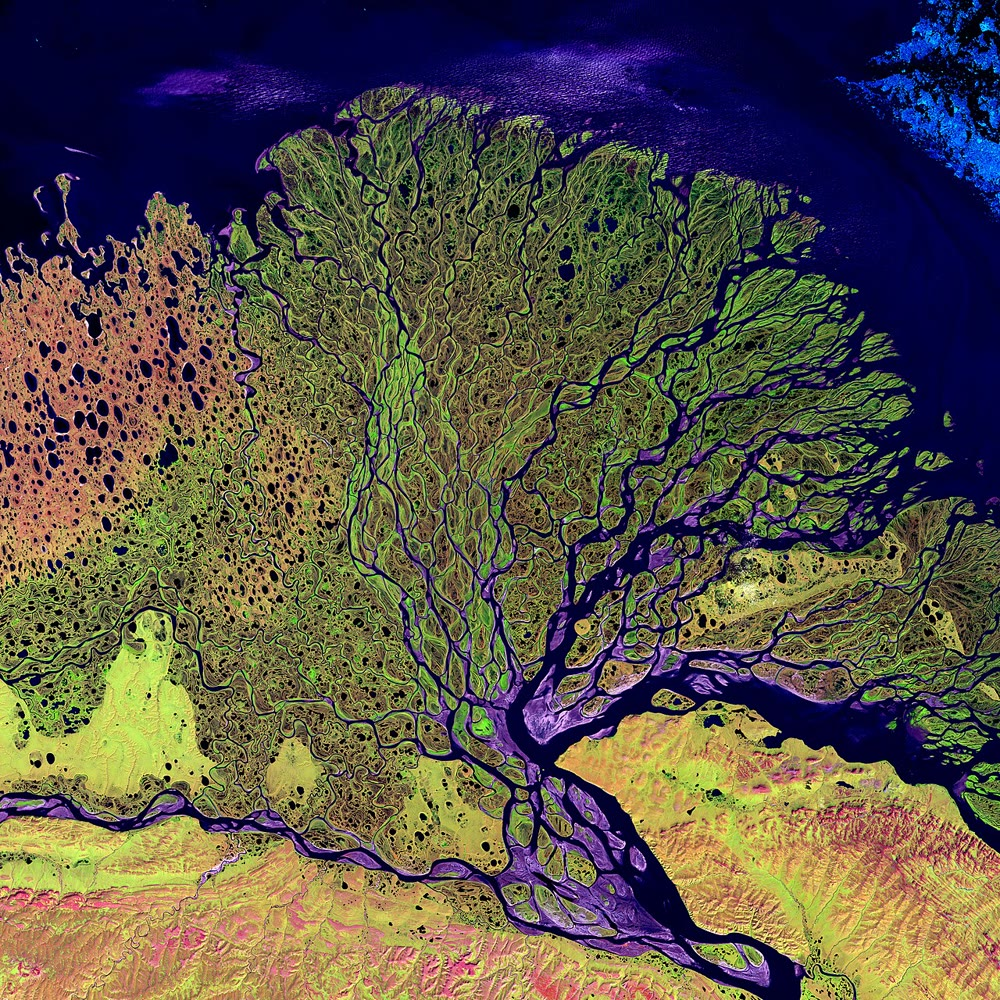
\includegraphics[width=\linewidth]{images/book1/g9-lena-delta.jpg}
\end{minipage}\hfill
\begin{minipage}[c]{0.46\linewidth}\raggedright
{\small \omterm{def:g5:water-shapes-the-land:delta}{دلتا} \omterm{def:g1:landscapes-around-us:water}{نهر} لينا، في سيبيريا، حيث يلتقي \omterm{def:g2:water-on-earth:ocean}{بالمحيط} المتجمد الشمالي:
صورة لاندسات بألوان زائفة التُقطت في 27~فبراير 2000، صُنعت بالأشعة تحت
الحمراء القصيرة الموجة والأشعة تحت الحمراء والضوء الأحمر. وتظهر قنوات
\omterm{def:g1:landscapes-around-us:water}{النهر} الكثيرة بالأزرق. مركز بيانات EROS التابع لهيئة المسح الجيولوجي
الأمريكية، عبر موقع «الأرض المرئية» لناسا (ملك عام، عبر ويكيميديا كومنز).}
\end{minipage}
% ledger: commons:lena-landsat
\label{fig:g9:maps-of-the-earth:lena}
\end{omfigure}

\section{تحديد الموقع بالأقمار الصناعية}

يستطيع هاتف أو سيارة أن يعرف موقعه بدقة بضعة أمتار، في أي مكان تقريبًا
من الأرض. وهو لا يرى الأقمار الصناعية؛ بل يصغي إليها.

\begin{definition}[تحديد الموقع بالأقمار الصناعية]\label{def:g9:maps-of-the-earth:positioning}
\emph{تحديد الموقع بالأقمار الصناعية}\index{تحديد الموقع بالأقمار الصناعية}
هو إيجاد موقع على الأرض انطلاقًا من المسافات إلى عدة أقمار صناعية مواقعها
معروفة. ويحسب المستقبِل كل مسافة من الزمن الذي تستغرقه إشارة القمر
الصناعي لتبلغه.
\end{definition}

يحافظ النظام الأمريكي، GPS، على 24 قمرًا صناعيًا عاملًا على الأقل على
\omterm{def:g4:world-physical-map:altitude}{ارتفاع} نحو \qty{20200}{km}. ويدور كل منها حول الأرض مرتين في اليوم، في
ستة مدارات موزعة حول الكوكب، بحيث تكون أربعة أقمار صناعية على الأقل في
مجال الرؤية من أي نقطة تقريبًا على الأرض. والإشارة الآتية من بعد
\qty{20200}{km}، المنتقلة بسرعة الضوء، تصل بعد $20\,200 \div
300\,000 \approx 0.067$~s: فيقيس المستقبِل هذا الزمن ويحوّله إلى
مسافة.
% ledger: gps:constellation, const:c (travel time computed in figdata/grade-9/trilateration.py)

كيف تعطي المسافات موقعًا؟ تصوّر الفكرة على \omterm{def:g2:drawing-to-map:map}{خريطة} مستوية. إذا كان المستقبِل
على بعد \qty{5}{km} من المحطة~A، فهو يقع في مكان ما على دائرة نصف قطرها
\qty{5}{km} حول A. وإذا كان أيضًا على بعد \qty{10}{km} من B، فهو يقع على
الدائرتين معًا: في إحدى النقطتين اللتين تتقاطعان فيهما. ومسافة ثالثة،
\qty{5}{km} من C، تختار النقطة الصحيحة. وفي الفضاء، تصير الدوائر كرات،
ويلزم قمر صناعي إضافي للسبب نفسه.

\begin{omfigure}
\begin{minipage}[c]{0.5\linewidth}\centering
\begin{tikzpicture}
\begin{axis}[x=0.42cm, y=0.42cm, xmin=-1, xmax=13, ymin=-1.5, ymax=13,
  ticks=none, axis line style={black!40}]
  \addplot[omSea!70!black, line width=0.6pt] table {figdata/out/grade-9-trilateration-circles.dat};
  \addplot[only marks, mark=triangle*, mark size=2.6pt, point meta=explicit symbolic, nodes near coords,
    nodes near coords style={font=\footnotesize\bfseries, anchor=south west, inner sep=1pt}]
    table[meta=label] {figdata/out/grade-9-trilateration-beacons.dat};
  % labels first (on a white patch), then the points on top of them
  \addplot[only marks, mark=none, point meta=explicit symbolic, nodes near coords,
    nodes near coords style={font=\footnotesize\bfseries, anchor=north east, xshift=-1pt, yshift=-1pt, inner sep=1pt, fill=white, text=red!75!black}, skip coords between index={1}{2}]
    table[meta=label] {figdata/out/grade-9-trilateration-points.dat};
  \addplot[only marks, mark=none, point meta=explicit symbolic, nodes near coords,
    nodes near coords style={font=\footnotesize, anchor=south west, xshift=1pt, yshift=1pt, inner sep=1pt, fill=white}, skip coords between index={0}{1}]
    table[meta=label] {figdata/out/grade-9-trilateration-points.dat};
  \addplot[only marks, mark=*, mark size=2pt, red!75!black, skip coords between index={1}{2}] table {figdata/out/grade-9-trilateration-points.dat};
  \addplot[only marks, mark=o, mark size=2pt, fill=white, skip coords between index={0}{1}] table {figdata/out/grade-9-trilateration-points.dat};
\end{axis}
\end{tikzpicture}
\end{minipage}\hfill
\begin{minipage}[c]{0.46\linewidth}\raggedright
{\small تحديد الموقع على \omterm{def:g2:drawing-to-map:map}{خريطة} مستوية (رسم تخطيطي؛ لم تُرسم الشبكة
بالكيلومترات). يبعد المستقبِل R مسافة \qty{5}{km} عن A، و\qty{10}{km} عن
B، و\qty{5}{km} عن C. وتتقاطع الدائرتان حول A وB في R وفي نقطة زائفة F؛
ولا تقع على الدائرة حول C إلا R.}
\end{minipage}
% ledger: (invented region: exercise data, figdata/grade-9/trilateration.py)
\label{fig:g9:maps-of-the-earth:trilateration}
\end{omfigure}

\begin{omfigure}
\begin{minipage}[t]{0.48\linewidth}\centering
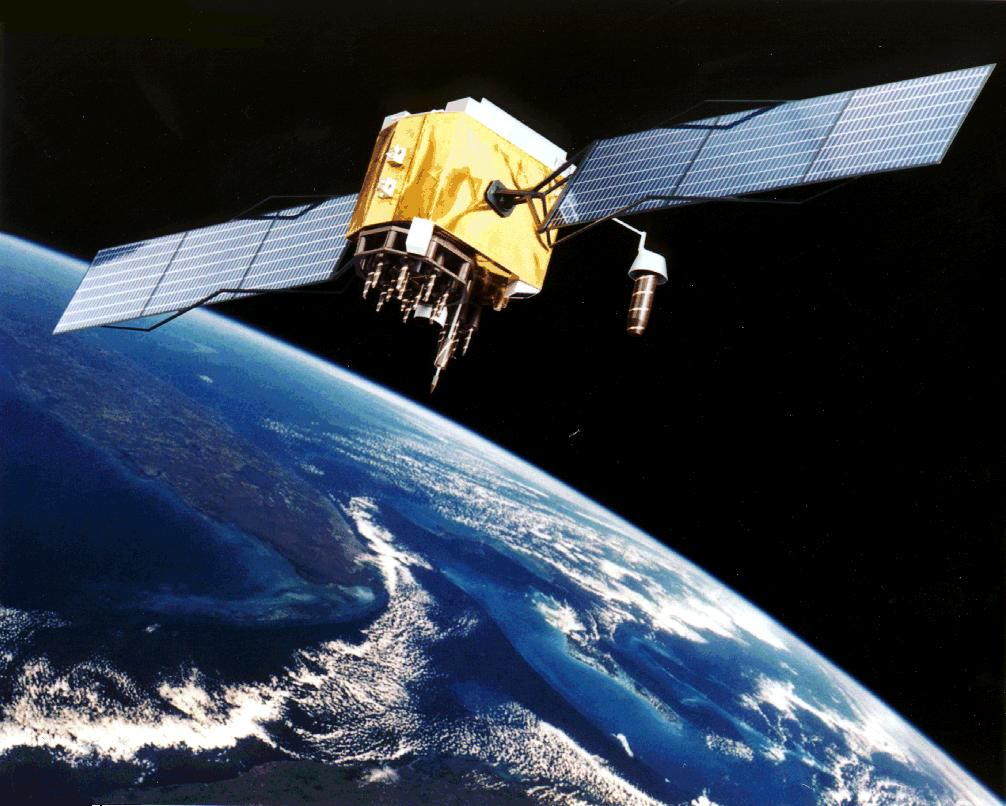
\includegraphics[width=\linewidth]{images/book1/g9-gps-satellite.jpg}

{\small قمر صناعي من أقمار GPS في مداره، كما تخيّله فنان. ناسا (ملك عام،
عبر ويكيميديا كومنز).}
\end{minipage}\hfill
\begin{minipage}[t]{0.48\linewidth}\centering
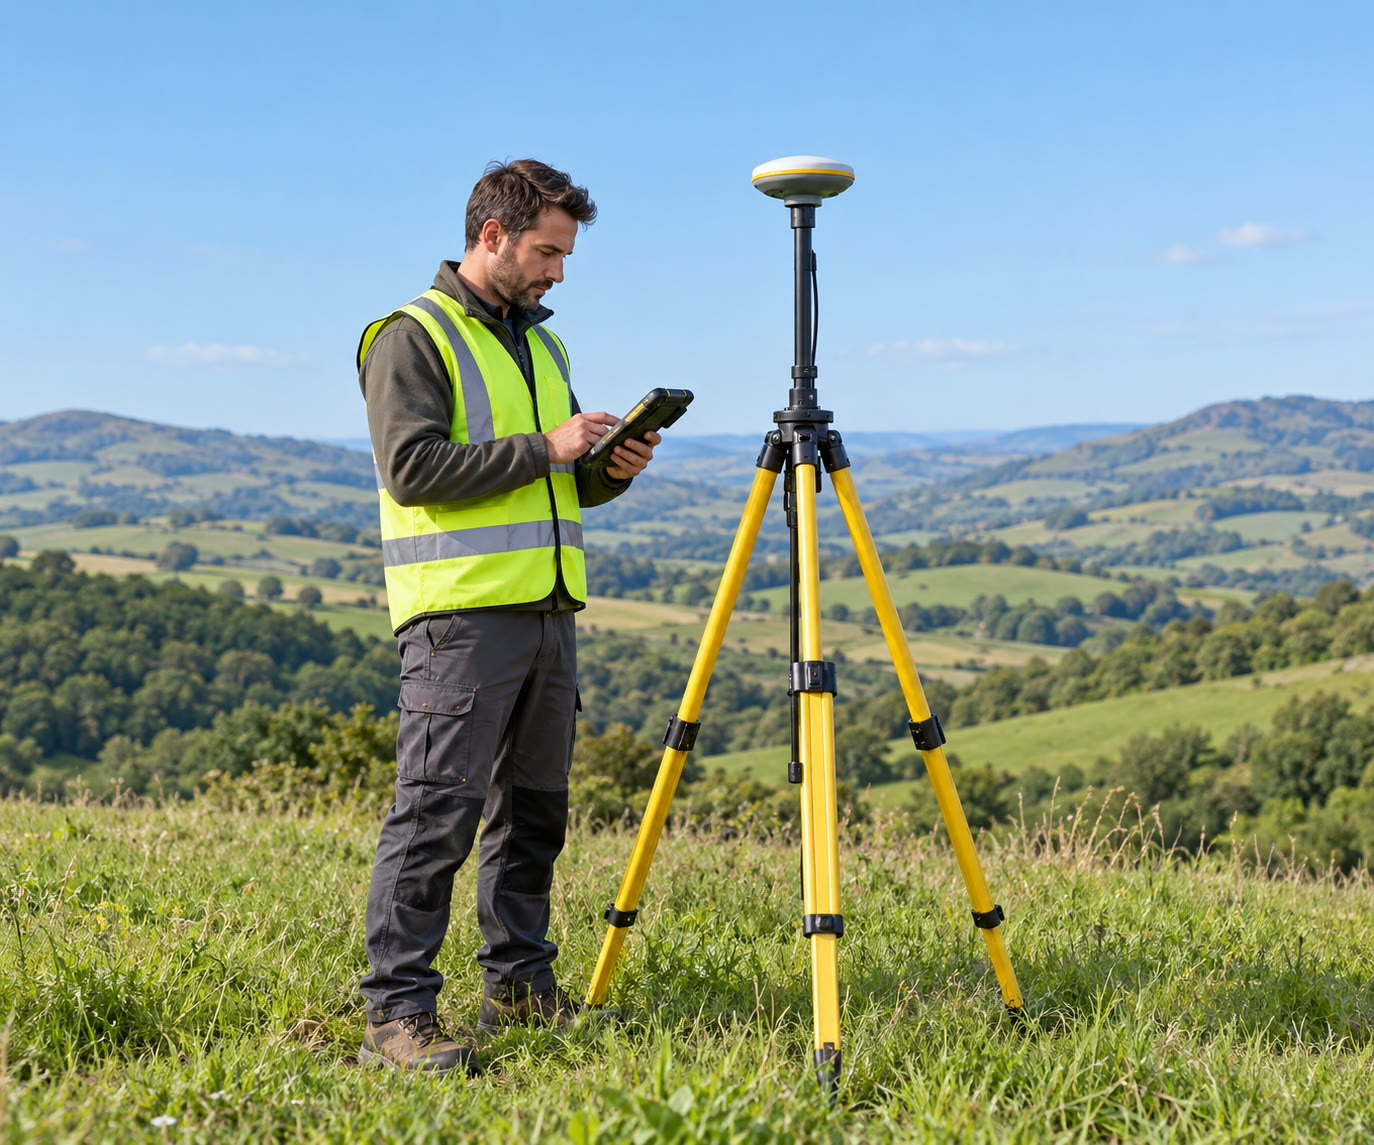
\includegraphics[width=\linewidth]{images/book1/ai/g9-surveyor.jpg}

{\small مسّاح يحدد موقع نقطة بمستقبِل للأقمار الصناعية مثبت على حامل
ثلاثي القوائم (رسم توضيحي).}
\end{minipage}
% ledger: commons:gps-iif
\label{fig:g9:maps-of-the-earth:gps}
\end{omfigure}

\section{تمارين}

\begin{exercise}[$\star$]\label{exo:g9:maps-of-the-earth:1}
أعطِ الكلمة المناسبة لكل وصف. (أ) قاعدة ترسل كل نقطة من الكرة الأرضية
إلى نقطة من \omterm{def:g2:drawing-to-map:map}{خريطة} مسطحة. (ب) خط يصل بين نقاط لها \omterm{def:g4:world-physical-map:altitude}{الارتفاع} نفسه. (ج) نسبة
مثل $1 : 50\,000$. (د) الفرق في \omterm{def:g4:world-physical-map:altitude}{الارتفاع} بين خطي كنتور متجاورين. (ه) رصد
الأرض من بعيد، من قمر صناعي
مثلًا.
\end{exercise}

\begin{exercise}[$\star$]\label{exo:g9:maps-of-the-earth:2}
حوّل كل مسافة على \omterm{def:g2:drawing-to-map:map}{الخريطة} إلى مسافة على الأرض، بالأمتار أو الكيلومترات.
(أ) \qty{4}{cm} على \omterm{def:g2:drawing-to-map:map}{خريطة} بمقياس $1 : 25\,000$. (ب) \qty{3}{cm} على
\omterm{def:g2:drawing-to-map:map}{خريطة} بمقياس $1 : 50\,000$. (ج) \qty{2.5}{cm} على \omterm{def:g2:drawing-to-map:map}{خريطة} بمقياس
$1 : 1\,000\,000$. (د) على \omterm{def:g2:drawing-to-map:map}{خريطة} بمقياس $1 : 25\,000$، كم سنتيمترًا يمثل \qty{1}{km}؟
\end{exercise}

\begin{exercise}[$\star$]\label{exo:g9:maps-of-the-earth:3}
صواب أم خطأ؟ صحّح الجمل الخاطئة. (أ) يمكن \omterm{def:g3:continents-and-oceans:world-map}{لخريطة العالم} أن تُظهر الأرض
كلها دون أن تشوّه أي شيء. (ب) في \omterm{def:g2:drawing-to-map:map}{خريطة} مركاتور، تبدو غرينلاند أكبر مما
هي. (ج) في \omterm{def:g2:drawing-to-map:map}{الخريطة} المتساوية المساحة، تُحفظ الأشكال في كل مكان. (د) يبقى
\omterm{def:g9:maps-of-the-earth:numerical-scale}{المقياس الخطي} صحيحًا حين تُكبَّر \omterm{def:g2:drawing-to-map:map}{الخريطة} في آلة
نسخ.
\end{exercise}

\begin{exercise}[$\star$]\label{exo:g9:maps-of-the-earth:4}
في \omterm{def:g9:maps-of-the-earth:topographic-map}{الخريطة الطبوغرافية}، (أ) ماذا يعني أن تكون خطوط الكنتور متقاربة جدًا؟
(ب) ومتباعدة؟ (ج) ماذا تُظهر خطوط الكنتور المغلقة التي يزداد ارتفاعها نحو
الداخل؟ (د) لماذا لا يمكن أن يتقاطع خطا كنتور أبدًا؟
\end{exercise}

\begin{exercise}[$\star\star$]\label{exo:g9:maps-of-the-earth:5}
% ledger: data:ne-land (factor 1/cos^2, figdata/grade-9/projections.py)
في \omterm{def:g2:drawing-to-map:map}{خريطة} مركاتور، تُكبَّر المساحات عند \omterm{def:g6:latitude-longitude:latitude}{خط العرض} \ang{60} أربع مرات، وعند
\omterm{def:g6:latitude-longitude:latitude}{خط العرض} \ang{30} نحو 1.33 مرة، مقارنةً \omterm{def:g3:continents-and-oceans:equator}{بخط الاستواء}. (أ) رُسمت على \omterm{def:g2:drawing-to-map:map}{الخريطة}
\omterm{def:g1:landscapes-around-us:water}{بحيرة} مساحتها \qty{1000}{km^2} عند \ang{60} شمالًا. فما المساحة الحقيقية
\omterm{def:g1:landscapes-around-us:water}{لبحيرة} عند \omterm{def:g3:continents-and-oceans:equator}{خط الاستواء} رُسمت بالحجم نفسه؟ (ب) جزيرتان لهما المساحة الحقيقية
نفسها تقعان عند \ang{30} وعند \ang{60}. كم مرة تبدو الثانية أكبر من
الأولى؟ (ج) لماذا لا تستطيع \omterm{def:g2:drawing-to-map:map}{خريطة} مركاتور أبدًا أن تُظهر
\omterm{def:g3:continents-and-oceans:poles}{القطبين}؟
\end{exercise}

\begin{exercise}[$\star\star$]\label{exo:g9:maps-of-the-earth:6}
% ledger: (invented region: the Varden Hills map of the chapter)
استعمل \omterm{def:g9:maps-of-the-earth:topographic-map}{الخريطة الطبوغرافية} لتلال فاردن في هذا الفصل. (أ) ما \omterm{def:g9:maps-of-the-earth:contour}{الفاصل
الكنتوري}؟ (ب) ما \omterm{def:g4:world-physical-map:altitude}{ارتفاع} القمة المعلَّمة بنقطة ارتفاعها، وما \omterm{def:g4:world-physical-map:altitude}{ارتفاع} \omterm{def:g9:maps-of-the-earth:contour}{خط
الكنتور} الرئيسي \omterm{def:g2:water-on-earth:ocean}{المحيط} بها مباشرة؟ (ج) يجري \omterm{def:g1:landscapes-around-us:water}{النهر} شرقًا. هل قاع \omterm{def:g1:landscapes-around-us:landform}{الوادي}
أعلى في غرب \omterm{def:g2:drawing-to-map:map}{الخريطة} أم في شرقها؟ (د) على طول C--D، شمال \omterm{def:g1:landscapes-around-us:water}{النهر}، بين أي
خطي كنتور تكون الخطوط أشد تقاربًا؟ وماذا يخبرك ذلك عن الانحدار
هناك؟
\end{exercise}

\begin{exercise}[$\star\star$]\label{exo:g9:maps-of-the-earth:7}
% ledger: (invented region: profile C--D, figdata/grade-9/varden_topo.py)
استعمل المقطع C--D في هذا الفصل. (أ) على أي \omterm{def:g4:world-physical-map:altitude}{ارتفاع} تقريبًا تقع C وD؟
(ب) ما أخفض \omterm{def:g4:world-physical-map:altitude}{ارتفاع} على طول المقطع، وكم يبعد عن C؟ (ج) ما طول قاع \omterm{def:g1:landscapes-around-us:landform}{الوادي}
المستوي على طول C--D؟ (د) رُسم المقطع بمقياس رأسي ممطوط ثلاث مرات. لماذا
يفعل راسمو الخرائط ذلك
كثيرًا؟
\end{exercise}

\begin{exercise}[$\star\star$]\label{exo:g9:maps-of-the-earth:8}
على \omterm{def:g2:drawing-to-map:map}{خريطة} بمقياس $1 : 25\,000$، يعبر درب \omterm{def:g9:maps-of-the-earth:contour}{خط الكنتور} \qty{200}{m} ثم \omterm{def:g9:maps-of-the-earth:contour}{خط
الكنتور} \qty{300}{m}، بعد \qty{2}{cm}. (أ) ما المسافة الأفقية بين
النقطتين على الأرض؟ (ب) بكم يصعد الدرب؟ (ج) ما الانحدار، نسبةً مئوية؟
(د) وبعد ذلك، يبعد خطا كنتور يفصل بينهما \qty{100}{m} في \omterm{def:g4:world-physical-map:altitude}{الارتفاع}
\qty{4}{cm} أحدهما عن الآخر على \omterm{def:g2:drawing-to-map:map}{الخريطة}. هل الدرب هناك أشد انحدارًا أم
ألطف؟ وبكم؟
\end{exercise}

\begin{exercise}[$\star\star$]\label{exo:g9:maps-of-the-earth:9}
% ledger: usgs:landsat1
كان لاندسات~1 يدور حول الأرض 14 مرة في اليوم ويمر فوق المكان نفسه كل 18
يومًا. (أ) كم مدارًا أكمل بين مرورين فوق المكان نفسه؟ (ب) كان كل مدار
يستغرق 103 دقائق. كم ساعة تستغرق 14 مدارًا؟ (ج) بُني ليعمل سنة واحدة،
فأُطفئ في 6~يناير 1978، بعد خمس سنوات ونصف من إطلاقه. كم ضعفًا من عمره
المقرر عمل؟ (د) اذكر تغيرًا واحدًا على سطح الأرض يمكن أن تُظهره صور المكان
نفسه الملتقطة بفارق
سنوات.
\end{exercise}

\begin{exercise}[$\star\star$]\label{exo:g9:maps-of-the-earth:10}
% ledger: gps:constellation, const:c
يبعد قمر صناعي من أقمار GPS نحو \qty{20200}{km}؛ وتنتقل إشارته بسرعة نحو
\qty{300000}{km} في الثانية. (أ) كم تستغرق الإشارة لتصل؟ اكتب الجواب
بالترميز العلمي. (ب) لو كانت ساعة المستقبِل مخطئة بمقدار
$1 \times 10^{-3}$~s، فما الخطأ في المسافة الناتج عن ذلك؟ (ج) ماذا يخبرك
ذلك عن الساعات المستعملة في \omterm{def:g9:maps-of-the-earth:positioning}{تحديد الموقع بالأقمار
الصناعية}؟
\end{exercise}

\begin{exercise}[$\star\star\star$]\label{exo:g9:maps-of-the-earth:11}
على \omterm{def:g2:drawing-to-map:map}{خريطة} مستوية ذات شبكة بالكيلومترات، تقع المحطة A عند $(0, 0)$
والمحطة B عند $(10, 0)$. ويبعد مستقبِل \qty{6}{km} عن A و\qty{8}{km} عن
B. (أ) بيّن أن النقطة $(3.6, 4.8)$ تبعد \qty{6}{km} عن A و\qty{8}{km} عن
B. (ب) أعطِ نقطة أخرى على المسافتين نفسيهما من A وB. (ج) تقع محطة ثالثة C
عند $(0, 10)$، ويبعد المستقبِل عنها نحو \qty{6.3}{km}. أي النقطتين هي
المستقبِل؟ (د) لماذا يحتاج \omterm{def:g9:maps-of-the-earth:positioning}{تحديد الموقع بالأقمار الصناعية} إلى عدة
أقمار؟
\end{exercise}

\begin{exercise}[$\star\star\star$]\label{exo:g9:maps-of-the-earth:12}
% ledger: data:ne-land (areas, figdata/grade-9/projections.py)
يغطي البر الإفريقي الرئيسي نحو 29~مليون~\unit{km^2} وغرينلاند نحو
2.1~مليون~\unit{km^2}. (أ) كم مرة تكون إفريقيا أكبر؟ (ب) في \omterm{def:g2:drawing-to-map:map}{خريطة} مركاتور،
تُكبَّر المساحات قرب وسط غرينلاند، عند نحو \ang{72} شمالًا، نحو 10.5 مرات.
قدّر المساحة التي تبدو لغرينلاند. (ج) تمتد إفريقيا على جانبي \omterm{def:g3:continents-and-oceans:equator}{خط الاستواء}،
حيث تُكبَّر المساحات قليلًا. قارن جوابك عن (ب) بمساحة إفريقيا، واشرح
\omterm{def:g2:drawing-to-map:map}{خريطة} الجدار في بداية الفصل. (د) أي إسقاط تختار لتُظهر مساحات \omterm{def:g3:continents-and-oceans:continent}{القارات}
بإنصاف؟
\end{exercise}

\section{مسألة: درب عبر تلال فاردن}

\begin{problem}[{مسألة نهاية الأسبوع --- رسم المخططون دربًا عبر تلال
فاردن على الخريطة الطبوغرافية؛ والجواب الأخير هو طول الدرب بالكيلومترات
ومجموع صعوده بالأمتار}]
\label{pb:g9:maps-of-the-earth:1}
% ledger: (invented region: the Varden Hills, figdata/grade-9/varden_topo.py, part problem: leg lengths 3.6 / 2.5 / 2.35 cm, spot heights 296 / 143 / 335 / 544 m, 4.2 km, 401 m)
يبدأ الدرب عند مزرعة S، وينزل إلى جسر B فوق \omterm{def:g1:landscapes-around-us:water}{النهر}، ثم يصعد إلى ملجأ W
ومنه إلى القمة T. وكل مرحلة مستقيمة، وهي إما تنزل فقط وإما تصعد فقط.
\omterm{def:g2:drawing-to-map:map}{والخريطة} بمقياس $1 : 50\,000$؛ وارتفاعات S وB وW وT مكتوبة
بجانبها.

\begin{omfigure}
\begin{tikzpicture}
\begin{axis}[x=1.6cm, y=1.6cm, xmin=2, xmax=8, ymin=1.8, ymax=6.2, ticks=none,
  axis line style={black!60}, clip mode=individual]
  \addplot[contour] table {figdata/out/shared-region-contours.dat};
  \addplot[index contour] table {figdata/out/shared-region-index-contours.dat};
  \addplot[river] table {figdata/out/shared-region-river.dat};
  \addplot[only marks, mark=none, point meta=explicit symbolic, nodes near coords,
    nodes near coords align={center}, nodes near coords style={font=\tiny, fill=white, inner sep=0.6pt, text=omContour}]
    table[meta=label] {figdata/out/grade-9-varden_topo-labels.dat};
  \addplot[red!75!black, line width=1pt, dashed] table[x=x_km, y=y_km] {figdata/out/grade-9-varden_topo-path.dat};
  \addplot[only marks, mark=*, mark size=1.6pt, red!75!black, point meta=explicit symbolic, nodes near coords,
    nodes near coords align={right}, nodes near coords style={font=\scriptsize\bfseries, text=black, fill=white, fill opacity=0.8, text opacity=1, inner sep=1pt}]
    table[meta=label] {figdata/out/grade-9-varden_topo-points.dat};
  \coordinate (na) at (axis cs:8.35,5.4);
\end{axis}
\pic at (na) {northarrow};
\end{tikzpicture}

{\small الدرب S--B--W--T على \omterm{def:g9:maps-of-the-earth:topographic-map}{الخريطة الطبوغرافية} لتلال فاردن (معروضة هنا
مصغّرة؛ وعلى \omterm{def:g2:drawing-to-map:map}{الخريطة} الأصلية بمقياس $1 : 50\,000$ تبلغ أطوال المراحل
3.6 و2.5 و\qty{2.35}{cm}).}
\label{fig:g9:maps-of-the-earth:path}
\end{omfigure}

\noindent\textbf{الجزء الأول --- المسار على الخريطة.}\par\nopagebreak
\begin{enumerate}[beginpenalty=10000]
  \item بمقياس $1 : 50\,000$، كم مترًا على الأرض يمثل \qty{1}{cm}
        من \omterm{def:g2:drawing-to-map:map}{الخريطة}؟
  \item على \omterm{def:g2:drawing-to-map:map}{الخريطة} الأصلية، تبلغ المرحلة S--B \qty{3.6}{cm}. فما طولها
        على الأرض، بالكيلومترات؟
  \item تبلغ المرحلتان B--W وW--T \qty{2.5}{cm} و\qty{2.35}{cm}.
        فما طولهما على الأرض؟
  \item في أي اتجاه عام يمتد الدرب من B إلى T؟
\end{enumerate}

\noindent\textbf{الجزء الثاني --- الصعود.}\par\nopagebreak
\begin{enumerate}[resume, beginpenalty=10000]
  \item ما \omterm{def:g9:maps-of-the-earth:contour}{الفاصل الكنتوري} \omterm{def:g2:drawing-to-map:map}{للخريطة}؟
  \item أي مرحلة تنزل؟ وبكم مترًا؟
  \item بكم مترًا يصعد الدرب في B--W، وفي W--T؟
  \item ما متوسط انحدار المرحلة W--T، نسبةً مئوية؟
  \item لماذا لم يرسم المخططون الدرب خطًا مستقيمًا من S
        إلى T؟
\end{enumerate}

\noindent\textbf{الجزء الثالث --- النزهة.}\par\nopagebreak
\begin{enumerate}[resume, beginpenalty=10000]
  \item افترض أن ماشيًا يقطع \qty{4}{km} في الساعة على الأرض المستوية
        ويحتاج إلى دقيقة إضافية لكل \qty{10}{m} من الصعود. كم تستغرق
        النزهة كلها؟
  \item تسلك ماشية أخرى الدرب في الاتجاه المعاكس، من T إلى S.
        كم مترًا تصعد؟
  \item ما الطول الكلي للدرب، بالكيلومترات، ومجموع صعوده،
        بالأمتار؟
\end{enumerate}
\end{problem}
